\documentclass[11pt,a4paper,oneside,titlepage]{article}

\usepackage[english]{babel}
\usepackage{lineno,hyperref}
\usepackage[nolist]{acronym}
\usepackage[onehalfspacing]{setspace}
\usepackage{booktabs}
\usepackage{float}
\usepackage{amsmath}
\usepackage{listings}
\usepackage{color}
\usepackage{hyperref}
\usepackage{graphicx}
\usepackage{blindtext}
\usepackage{datetime}

\definecolor{LightGray}{gray}{0.70}
\lstdefinestyle{MctCpp}{%
    language=C++,
    keywordstyle=\bfseries,
    commentstyle=\itshape,
    rangeprefix=//--,rangesuffix=--,
    includerangemarker=false,
    columns=spaceflexible,
    escapeinside={/*@}{@*/},
    tabsize=4,
    frame=leftline,
    rulecolor=\color{LightGray},
    basicstyle=\ttfamily,
    numbers=left,
    numberstyle=\normalfont\tiny\color{LightGray},
    xleftmargin=0.75cm,
}

\lstdefinestyle{MctTxt}{%
    language={},
    keywordstyle=\bfseries,
    commentstyle=\itshape,
    rangeprefix=//--,rangesuffix=--,
    includerangemarker=false,
    columns=spaceflexible,
    escapeinside={/*@}{@*/},
    tabsize=4,
    frame=leftline,
    rulecolor=\color{LightGray},
    basicstyle=\ttfamily,
    numbers=left,
    numberstyle=\normalfont\tiny\color{LightGray},
    xleftmargin=0.75cm,
}

\textheight = 25cm
\textwidth = 15cm

\hoffset = -1cm
\voffset = -2cm


\begin{document}
%------------------------------------------------------------------------------
\newcommand{\CenFig}[2]{
    \begin{figure}[H]
        \begin{center}
            \includegraphics[width=#2\textwidth]{#1}
        \end{center}
    \end{figure}
}

\makeatletter
\lst@Key{matchrangestart}{f}{\lstKV@SetIf{#1}\lst@ifmatchrangestart}
\def\lst@SkipToFirst{%
    \lst@ifmatchrangestart\c@lstnumber=\numexpr-1+\lst@firstline\fi
    \ifnum \lst@lineno<\lst@firstline
        \def\lst@next{\lst@BeginDropInput\lst@Pmode
        \lst@Let{13}\lst@MSkipToFirst
        \lst@Let{10}\lst@MSkipToFirst}%
        \expandafter\lst@next
    \else
        \expandafter\lst@BOLGobble
    \fi}
\makeatother
%------------------------------------------------------------------------------
\newcommand{\FigCapLabSca}[4]{
\begin{figure}[H]
    \begin{center}
        \includegraphics[width=#4\textwidth]{#1}
        \caption[]{#2}
        \label{#3}
    \end{center}
\end{figure}
}
%
\thispagestyle{empty}
\begin{center}
    \begin{huge}
        \textbf{Technical Specifications\\The Big LebowSky}
    \end{huge}
    \begin{figure}[H]
        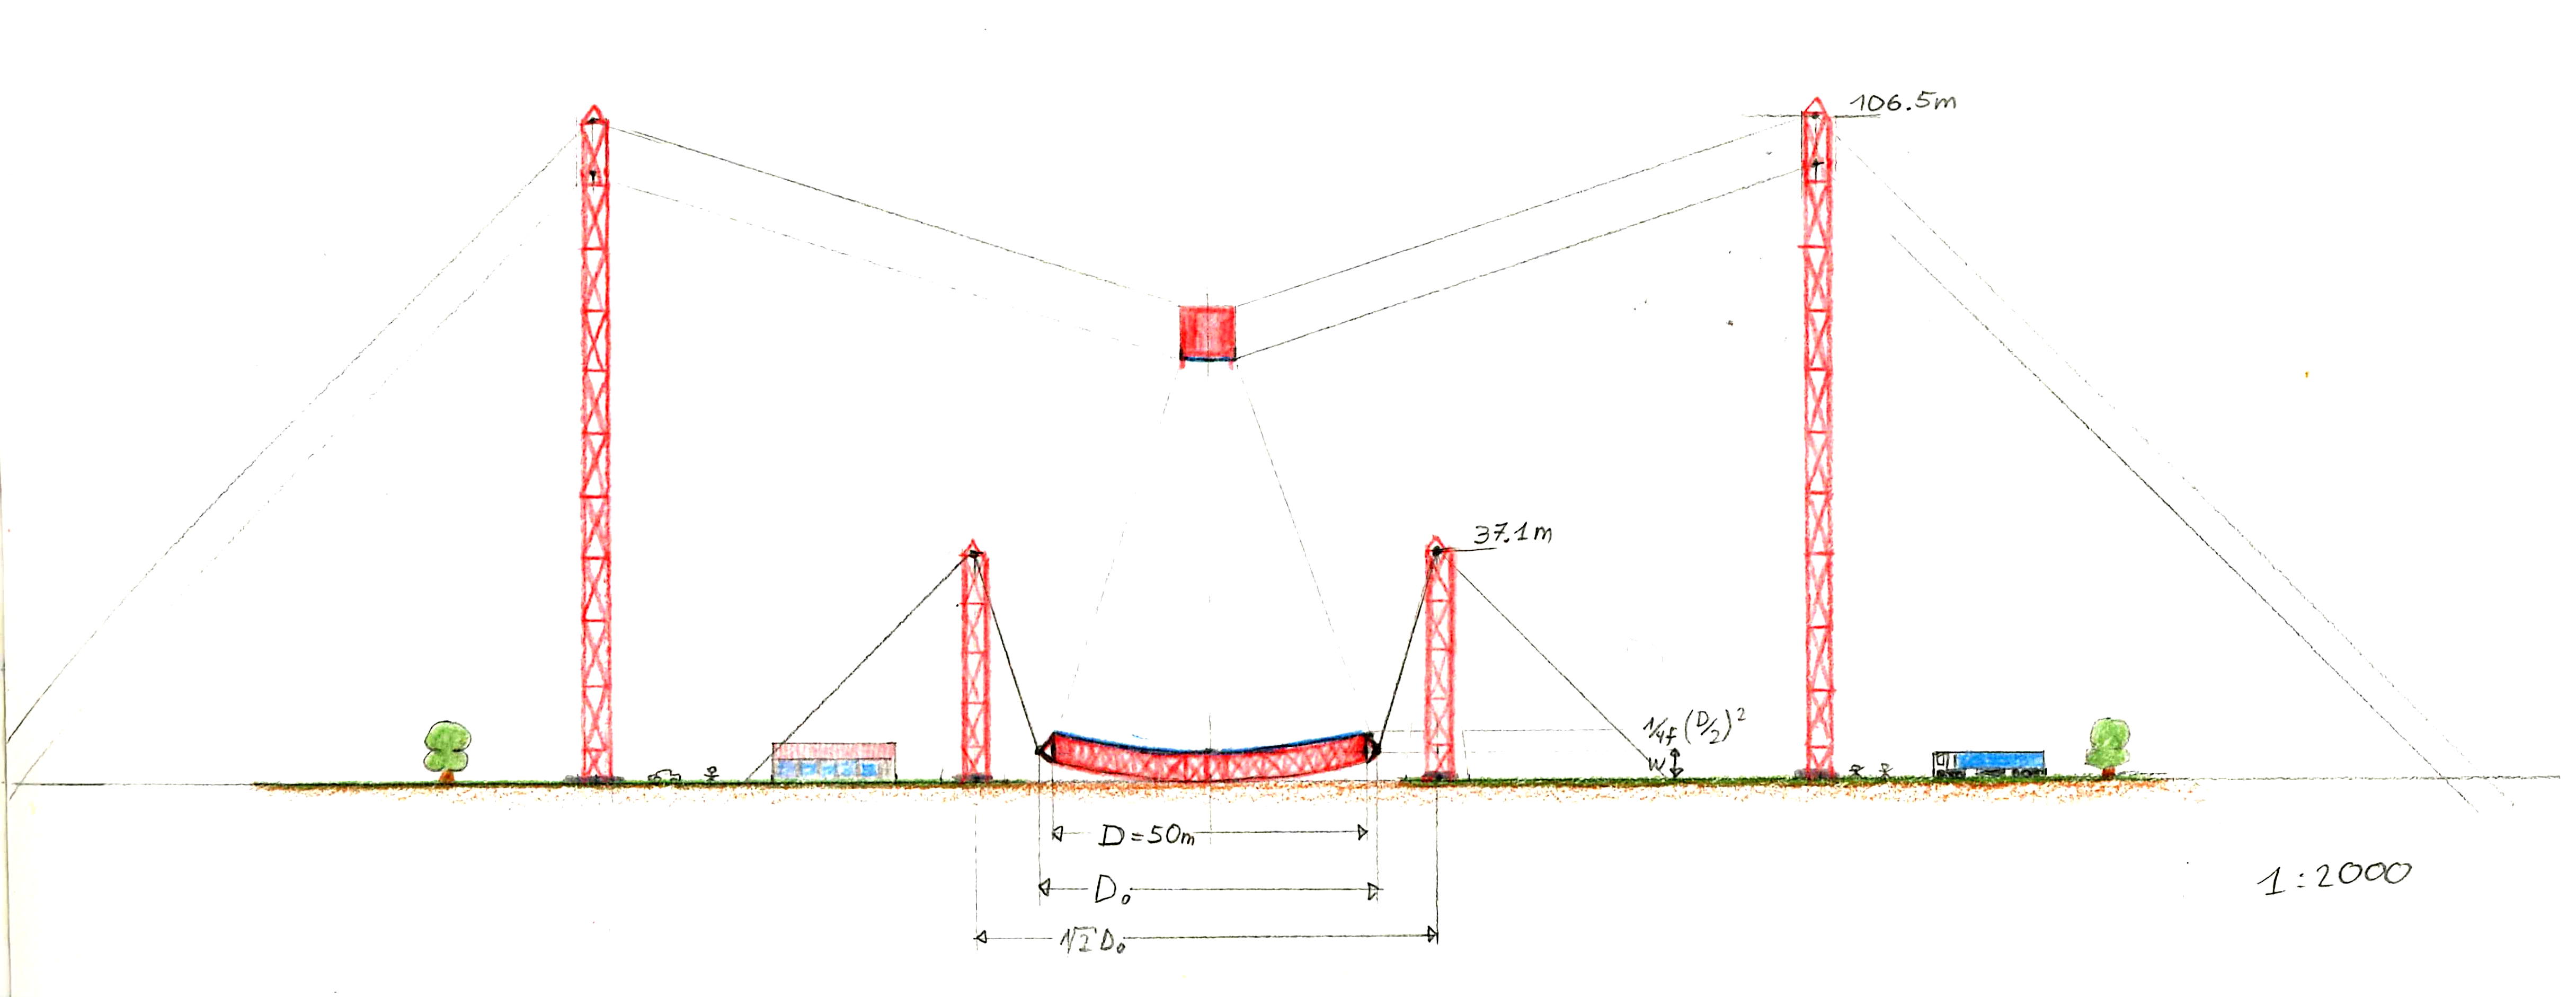
\includegraphics[width=1.0\textwidth]{figures/lebowsky_drawing.png}
    \end{figure}
    \vfill
    by\\
    \begin{Large}
        Sebastian Achim Mueller\\Dominik Neise\\Max Ludwig Ahnen\\
    \end{Large}
    sebmuell@phys.ethz.ch\\
    \vspace{20pt}
    Institute for Particle Physics
    \par\smallskip\noindent
    ETH Zurich\\ \today \\ \currenttime
\end{center}
\newpage
%-------------------------------------------------------------
\pagenumbering{Roman}
\tableofcontents
%-------------------------------------------------------------
\cleardoublepage
%
\setcounter{page}{0}
\pagenumbering{arabic}
%
\linenumbers
\newcommand{\OutOfFocus}{\textit{out of focus}}
\newcommand{\InFocus}{\textit{in focus}}
\newcommand{\FocalRatio}{F}
\newcommand{\FocalLength}{f}
\newcommand{\ImageDistance}{b}
\newcommand{\ImageSensorDistance}{d}
\newcommand{\ObjectDistance}{g}
\newcommand{\ApertureDiameter}{D}
\newcommand{\ApertureFunction}{A}
\newcommand{\BokehFunction}{B}
\newcommand{\FieldOfView}{\alpha}
\newcommand{\BokehRadius}{r_\BokehFunction}
\newcommand{\BokehTemplateFunction}{\BokehFunction_{\text{template}}}
\newcommand{\ApertureRadius}{r_\ApertureFunction}
\newcommand{\zHy}{{z_\text{Hy}}}
\newcommand{\zPa}{{z_\text{Pa}}}
\newcommand{\zDC}{{z_\text{DC}}}
%-------------------------------------------------------------------------------
\section{Site Selection}
%
The Telescope shall be located at high altitude e.g. 5000\,m a.s.l. on the ALMA telescope site in Chile.
%
First this is because at high altitudes less Cherenkov light from the air showers is absorbed in the atmosphere, which allows to have the lowest cosmic ray energy threshold possible.
%
Second, the 3D reconstruction power of the Telescope vanishes for features which are far above the aperture.
%
So we bring the Telescope as close as possible up to the air showers and the Cherenkov light production altitudes.
%
Also the site shall have dark night skies without arificial light polution.
%
Since most cosmic objects we want to observe are in the Milky Way's plane or center, we want a site on the southern hemisphere to have low zenith distances during observation.
%-------------------------------------------------------------------------------
\section{Target Geometry}
%
Here we define the most desireable target geometry of the telescope. 
%
All active actuators, which are moving the dish and the image sensor, should try to reach the target geometry during operation. 
%
We define all components relevant for the optics in the reflector frame. The $x$-$y$ plane in the origin of the reflector frame is called principal aperture plane. 
%
Along the $z$ axis is the optical axis of the refelctor.
%
Table \ref{TabBasicDimensions} shows the basic relative dimensions of the telescope.
%
Fix design keys of the telescope are its focal ratio of $\FocalLength/\ApertureDiameter = 1.5$ and its field of view of $6.5^\circ\,$.  
%
\begin{table}[H]
    \begin{center}
        \begin{tabular}{lr}
            \toprule
            aperture diameter $\ApertureDiameter$ & $100\,$a.u.\\
            focal length $\FocalLength$ & $150\,$a.u.\\
            F-number or foacal ratio, $\FocalLength/\ApertureDiameter$ & $1.5$\\
            image sensor distance $\ImageSensorDistance$ & $159.7\,$a.u.\\
            image sensor diameter & $17\,$a.u.\\
            image sensor housing diameter & $20.4\,$a.u.\\
            image sensor field of view $\FieldOfView$ & $6.5^\circ\,$\\
            \bottomrule
        \end{tabular}
        \caption[]{Basic telescope dimensions in arbitrary units (a.u.)}
        \label{TabBasicDimensions}
    \end{center}
\end{table}
%
The image sensor distance
%
\begin{eqnarray}
\ImageSensorDistance &=& \frac{1}{\frac{1}{\FocalLength} - \frac{1}{\ObjectDistance}}
\end{eqnarray}
%
depends on the absolute target object distance of about $g \approx 2500\,$m.
%
So a telescope of $\ApertureDiameter = 50\,$m will have $\ImageSensorDistance = 77.3\,$m and a $\ApertureDiameter = 100\,$m telescope will have $\ImageSensorDistance = 159.7\,$m
%
\subsection{Imaging Reflector}
%
We use a segmented imaging reflector with identical facets.
%
All mirror facets have the same hexagonel aperture and focal lenght $f$.
%
The $x$ and $y$ position of a mirror facet are defined by the hexagonal grid of the facets.
\CenFig{figures/2D_mirror_facets.png}{0.4}
%
The relative $z$ components of the mirror facets are defined by a parabolic component
%
\begin{eqnarray}
    \zPa(r) &=& \frac{1}{4 \FocalLength} r^2,
\end{eqnarray}
%
which depends on the facet's distance to the optical axis $r$.
%
A global offset $q$ is added so that the position of the $i$-th facet is 
%
\begin{eqnarray}
\label{eq_mirror_position}
\vec{m}_{i} &=& \begin{pmatrix}   
                            r_i \cos(\varphi_{i})\\
                            r_i \sin(\varphi_{i})\\
                            \zPa_{i}(r_i) + q 
                        \end{pmatrix}.
\end{eqnarray}
%
\FigCapLabSca{figures/mirror_facet_position_z.png}{$z$ positions of the facets}{FigFacetZ}{0.8}
%
The common offset $q$ is chosen so that the average distance between all the $N$ facet centers $\vec{m}$ and the focal point $\vec{\FocalLength} = (0,0, \FocalLength)^T$ becomes the focal lenght
%
\begin{eqnarray}
    \label{eq_correct_focus}
    \FocalLength &\stackrel{!}{=}& \frac{1}{N} \sum_{i}^N 
    %
    \left \vert 
    %
    \vec{m}_{i}- \vec{\FocalLength}\,
    %
    \right \vert.
    %
\end{eqnarray}
%
The facet orientations along the $z$ axis is defined by the hexagonal grid of the facets.
%
The $x$ and $y$ orientations are chosen so that the $i$-th mirror facet surface normal
%
\begin{eqnarray}
\label{eq_facet_normal}
\vec{n}_{i} &=& \frac{2\vec{\FocalLength} - \vec{m_i}}{\vert 2\vec{\FocalLength} - \vec{m_i} \vert}
\end{eqnarray}
%
is pointing towards the $2 \vec{\FocalLength}$ point.
%
\CenFig{figures/mirror_facet_orientation.png}{0.8}
%
\subsection{Restricted volumes}
%
To not reduce the effective aperture area of the telescope, some volumes should be kept free of obstacles.
%
Figure \ref{FigRestrictedArea} shows the restricted volumes on the telescope in yellow.
%
There is a blind cone in the center of the reflector which can be blocked to have additional support structures, see also Figure \ref{FigBlindApertureCenter}.
%
Support structres, that have to be in the restricted volumes, should be shaped so that the shadowing is minimal, e.g. using steel cables or flat structures which are elongated along the optical axis.
%
\FigCapLabSca{figures/lebowsky_restricted_areas.png}{
    Objects in the yellow area will reduce the effective aperture area. The more intense the yellow is, the more important it is to keep this region free. Figure is to scale, aperture diameter is 100\,a.u.
}{FigRestrictedArea}{0.68}
%
\subsection{Mirror Facets}
%
All mirror facets are the same and are interchangeable with each other.
%
The imaging mirror facets have a focal lenght $\FocalLength$ and a hexagonal shaped aperture.
%
Table \ref{TabFacets} shows mirror facets and their properties of some telescopes. 
%
We will adopt the hexagonal CTA LST mirror facets since they are the biggest facets which have proven to be mass producible today.
%
The weight of a two axis actuator for the facets is $\approx 5\,$kg/facet regardless of the size of the facet.
%
\begin{table}[H]
    \begin{center}
        \begin{tabular}{lccrrrrr}
            type designation & shape & $A$[m$^2$] & $s$[m] & $m$[kg] & $\rho_A$[kg/m$^2$] & $\rho_A$[kg/m$^2$]\\
             & & & & & raw & with actuators\\
            \toprule
            MAGIC 1st gen. & square & 0.25 & 0.50  & 4.0 & 16.0 & 21.0\\
            MAGIC 2nd gen. & hex    & 0.96 & 0.96 & 13.4 & 14.0 & 19.2\\
            VERITAS        & hex    & 0.32 & 0.61 & 10.4 & 32.4 & 48.0\\
            FACT/HEGRA     & hex    & 0.32 & 0.61 & 5.5 & 17.6 & 33.7\\
            CTA MST INAF   & hex    & 1.25 & 1.20 & 25.0 & 20.0 & 24.0\\
            CTA LST INAF   & hex    & 1.97 & 1.50 & 45.0 & 22.8 & 25.3\\
            \bottomrule
        \end{tabular}
        \caption[]{Typical mirror facets on IACTs. $s$ is the spacing of the facets, i.e. the flat to flat diameter of the hexagonal facets.}
        \label{TabFacets}
    \end{center}
\end{table}
%
\subsection{Imaging Sensor}
%
The shape of the image sensor is circular. It has pixel apertures of \mbox{$\Delta \alpha \approx 0.067^\circ$}.
%
The image sensor diameter 
%
\begin{eqnarray}
D_\text{sensor} &=& 2 \FocalLength \tan \left( \frac{\FieldOfView} {2}\right)
\end{eqnarray}
%
is defined by the desired field of view $\FieldOfView$ and the focal length $\FocalLength$. 
%
We expect the image sensor housing to have an size overhead of $120\%$. 
%
For $\ApertureDiameter=100\,$a.u. this yields to \mbox{$D_\text{sensor} = 17.04\,$a.u.} and a housing diameter of \mbox{$D_\text{sensor housing} = 20.45\,$a.u.}
%
We expect the electric compartment of the image sensor to be rather flat, maybe $2\,$a.u. to $4\,$a.u. in height.
%
The cylindrical image sensor housing is only as tall as it is width, because of the robo-crane mount in order to tilt the image sensor.
%
The sensor part itself is more like a flat disc.
%
Table \ref{TabFullImageSensors} shows typical image sensor dimensions of IACTs.
%
For the sensor electronic part, we expect our image sensor to be as lightweight as the lightest IACT image sensor units, which is about $\rho_A = 550\,$kg/m$^2$.
%
However, because of the height of the image sensor housing for the robo-crane mount we better be conservative and expect it to be heavy as $\rho_A = 1000\,$kg/m$^2$. 
%
\begin{table}[H]
    \begin{center}
        \begin{tabular}{lccrrrrr}
            type designation & $A$[m$^2$] & $m$[kg] & $\rho_A$[kg/m$^2$]\\
            \toprule
            CAT France & 0.19 & 110 & 560\\
            MAGIC      & 0.85 & 450 & 530\\ 
            VERITAS    & 0.42 & -- & -- \\ 
            FACT       & 0.12 & 175 & 1458\\
            HESS 1     & 1.35 & 800 & 593\\ 
            HESS 2     & 3.14 & 2800 & 891\\ 
            \bottomrule
        \end{tabular}
        \caption[]{Typical image sensor dimensions of IACTs including all housing components.}
        \label{TabFullImageSensors}
    \end{center}
\end{table}
%-------------------------------------------------------------------------------
\section{Geometry Margins}
%
The novel image sensor of this telescope will allow some misalignments and displacements between the image sensor and the imaging reflector.
%-----------
\subsection{Image Sensor relative to Reflector}
%-----------
\subsubsection{$z$ displacement}
%
The deviation in $z$ direction of the image sensor distance to its target distance
%
\begin{eqnarray}
\Delta \ImageSensorDistance & = & \ImageSensorDistance_\text{actual} -\ImageSensorDistance_\text{target}
\end{eqnarray}
%
may vary since our novel image sensor is able to reconstruct the effect when $\ImageSensorDistance_\text{actual}$ is known.
%
\CenFig{figures/image_sensor_displacement_z.png}{0.6}
%
\begin{table}[H]
    \begin{center}
        \begin{tabular}{lr}
            image sensor displacement $z$ & $\Delta \ImageSensorDistance$ [a.u.]\\
            \toprule
            Mandatory & -4.6 $<$ $\Delta \ImageSensorDistance$ $<$ 7.9\\
            Good      & -2.3 $<$ $\Delta \ImageSensorDistance$ $<$ 3.8\\
            Perfect   & -1.1 $<$ $\Delta \ImageSensorDistance$ $<$ 1.9\\
            \bottomrule
        \end{tabular}
    \end{center}
\end{table}
%-----------
\subsubsection{$x$, $y$ displacement}
%
An image sensor offset $\Delta xy$ to the optical axis can be accepted, when the $x$ and $y$ position of the image sensor with respect to the imaging reflector are known.
%
\CenFig{figures/image_sensor_displacement_xy.png}{0.6}
%
\begin{table}[H]
    \begin{center}
        \begin{tabular}{lr}
            image sensor displacement $x$, $y$ & $\Delta xy$ [a.u.]\\
            \toprule
            Mandatory & $< 0.72$\\
            Good      & $< 0.36$\\
            Perfect   & $< 0.18$\\
            \bottomrule
        \end{tabular}
    \end{center}
\end{table}
%-----------
\subsubsection{misalignment $x$, $y$}
%
A misalignment $\beta$ of the imaging reflector optical axis against the image sensor optical axis can be accepted, when $\beta$ is known.
%
Our novel image sensor is still able to reconstruct the image as recorded by well aligned image sensor.
%
However, we lose effective aperture area $A_\text{eff}$, since our image sensor has a view cone restriction of which is just enough to fit the aperture once.
%
\CenFig{figures/image_sensor_misalignment_xy_view_cone.png}{0.6}
%
\begin{table}[H]
    \begin{center}
        \begin{tabular}{lrr}
            image sensor misalignment $x$, $y$ & $\beta$ [deg] & $A_\text{eff}$ [\%]\\
            \toprule
            Mandatory & $< 3.0$ & 90.0\\
            Good      & $< 1.5$ & 95.0\\
            Perfect   & $< 0.75$ & 97.5\\
            \bottomrule
        \end{tabular}
    \end{center}
\end{table}
%-----------
\subsubsection{misalignment in $z$}
%
The image sensor may be arbitrarily rotated along the $z$ axis, as long as the rotations is known.
%-----------
\subsection{Image Sensor}
%
The image sensor itself is assumed to be stiff, i.e. the image sensor plane does not bend or deform more than $0.05\,$a.u. across its diameter.
%-----------
\subsection{Reflector Deformation}
%
As a rule of thumb:
The actual tilt of a mirror facet against its target tilt, caused by deformations of the dish, shall not exceed \mbox{$\frac{\Delta \alpha}{2} \approx 0.034^\circ$}, i.e. half the image sensor pixel size.
%
\begin{eqnarray}
\arccos \left( \vec{n}_\text{target} \cdot \vec{n}_\text{actual} \right) &<& \frac{\Delta \alpha}{2}
\end{eqnarray}
%-----------
\subsubsection{Slow and predictable Deformations}
%
When using mirror facet actuators, we can accept slow and predictable deformations of the dish support structure which even exceed $\frac{\Delta \alpha}{2}$, as they might be caused by gravitational slump.
%
Here slow means, that the mirror actuators can easily keep up with the deformations of the dish while the telescope is slowly tracking a source.
%
(The MAGIC actuators can tilt a facet with $0.5^\circ/$s).
%
Predictable means, that the deformation will always be the same for a given telescope orientation, so that they can be learned once and then be applied later. (This is what is successfully done on the MAGIC telescope).
%
In case there are no deformations above $\frac{\Delta \alpha}{2}$ anyhow, we might drop the mirror facet actuators, which would simplify the maintenance of the telescope a lot and also reduce its initial cost.
%-----------
\subsubsection{Unforeseen Deformations}
%
Deformations of the reflector dish by e.g. wind can not be foreseen. In general, the relative additional tilts of the facets shall not exceed \mbox{$\frac{\Delta \alpha}{2} \approx 0.034^\circ$}.
%
We can perform ray tracing simulations of the deformed dishes to see the effect on the imaging performance.
%
We might set up a feedback loop of mechanical deformation simulations and optical simulations. 
%-------------------------------------------------------------------------------
\section{Movements}
%<
The telescope has two different modes of movements during operation.
%
A slow mode to observe sources on the sky dome, and a fast mode to switch between the sources.
%
We want to avoid singularities in the inverse kinematics near the zenith.
%
For example ,the zenith singularity on the classic Altitude-Azimuth mount hinders fast repositioning.
%-----------
\subsection{Fast Repositioning}
%
When the telescope is pointing to a different source on the sky dome, the image sensor is not recording.
%
During the fast repositioning, the target geometry does not need to be fulfilled.
%
A high speed repositioning of $90^\circ/$min will enable gamma ray burst hunting, which would be a nice to have but is not mandatory.
%
\begin{table}[H]
    \begin{center}
        \begin{tabular}{lr}
            Fast Repositioning velocity & $\dot{\Theta}$[deg/min]\\
            \toprule
            Mandatory & 9\\
            Good      & 30\\
            Perfect   & 90\\
            \bottomrule
        \end{tabular}
    \end{center}
\end{table}
%-------------------------------------------------------------------------------
\subsection{Slow Tracking}
%
When the telescope is slowly tracking a source on the sky dome, it is only counteracting the rotation of the earth \mbox{$\dot{\Theta}_\text{Earth} = 0.25^\circ/$min}.
%
During slow tracking, the telescope has to try to reach its target geometry.
%
The telescope image sensor is only recording air showers in the slow tracking mode.
%
For some observations, it is useful to move around a source in a spiral movement, which demands for telescope tracking velocities $\dot{\Theta}$ which are three times higher than $\dot{\Theta}_\text{Earth}$.
%
\begin{table}[H]
    \begin{center}
        \begin{tabular}{lr}
            Tracking velocity & $\dot{\Theta}$[deg/min]\\
            \toprule
            Mandatory & 0.25\\
            Good      & 0.5\\
            Perfect   & 0.75\\
            \bottomrule
        \end{tabular}
    \end{center}
\end{table}
%-----------
\subsection{Range}
%
For the full azimuth range, the telescope should reach zenith distances $\Theta$ as high as $45\,^\circ$. 
%
\begin{table}[H]
    \begin{center}
        \begin{tabular}{lr}
            Zenith distance & $\Theta$ [deg]\\
            \toprule
            Mandatory & 30\\
            Good      & 45\\
            Perfect   & 60\\
            \bottomrule
        \end{tabular}
    \end{center}
\end{table}
%-------------------------------------------------------------------------------
\section{Geometry Tracking}
%
All displacements and misalignments of the image sensor with respect to the imaging reflector can only be accepted when we can track the actual position and orientation of the image sensor relative to the reflector.
%
We need a sampling rate to track these displacements and misalignments, one order of magnitude higher than the dominant eigenfrequencies of the structure. 
%
The MAGIC telescope arch has a eigenfrequency of $\approx 1\,$Hz. Assuming that the dominant eigenfrequencies on our big telescope will not be higher, a sampling rate $f_\text{sample}$ of $10\,$Hz might be sufficient.
%
\begin{table}[H]
    \begin{center}
        \begin{tabular}{lr}
            Sampling rate & $f_\text{sample}$ [Hz]\\
            \toprule
            Mandatory & 10\\
            Good      & 25\\
            Perfect   & 50\\
            \bottomrule
        \end{tabular}
    \end{center}
\end{table}
%
\begin{table}[H]
    \begin{center}
        \begin{tabular}{lr}
            image sensor $x$, $y$ and $z$ tracking accuracy & [a.u.]\\
            \toprule
            Mandatory & $\pm$ $7.2 \cdot 10^{-3}$\\
            Good      & $\pm$ $3.6 \cdot 10^{-3}$\\
            Perfect   & $\pm$ $1.8 \cdot 10^{-3}$\\
            \bottomrule
        \end{tabular}
    \end{center}
\end{table}
%
\begin{table}[H]
    \begin{center}
        \begin{tabular}{lr}
            image sensor tilt in $x$, $y$ ($\beta$), and $z$ tracking accuracy & [deg]\\
            \toprule
            Mandatory & $\pm$ 0.03\\
            Good      & $\pm$ 0.015\\
            Perfect   & $\pm$ 0.0075\\
            \bottomrule
        \end{tabular}
    \end{center}
\end{table}
%
A tracking implementation must be able to work at night without artificial illumination.
%
No light in the wavelength range of $200\,$nm to $1200\,$nm shall be emitted to track the positions, otherwise the image sensor will be blinded.
%
If artificial illumination is mandatory for the tracking, the duty cycle of the illumination system shall be as small as possible, best below $1\%$. 
%-------------------------------------------------------------------------------
\section{Maintanace}
%
Since the surfaces of the mirror facets degrade over time and the actuators of the facet will break over time, the mirror facets shall be reachable from below for maintenance.
%-------------------------------------------------------------------------------
\section{Threat due to sunlight}
%
The main imaging reflector dish of the telescope can be a threat when it projects the image of the sun on near by objects.
%
For a focal ratio of 1.5, the imaging reflector can project an image of the sun with up to $6\,$MW/m$^2$.
%
\begin{eqnarray}
\frac{I_\text{sun image}}{I_\text{solar constant}} = \frac{_\text{aperture area}}{_\text{image area}} = \frac{(D^2/4) \pi}{(D F \tan(0.25^\circ))^2 \pi} 
\end{eqnarray}
%
When we go for a telescope mount where the image sensor is mounted independent of the imaging reflector, we can profit from separating the image sensor from the dish to park it in a save position.
%
As long as the imaging reflector lies flat on the ground, it can not incinerate objects on the ground.
%
However, it might still heat up the nearby support structures.
%
We favor solutions which do not need additional mechanics, like e.g. domes or lids.
%-------------------------------------------------------------------------------
\section{Price Estimates}
%
The CTA mirror facets cost about 3000\,EUR/m$^2$ including the actuators.
%
The raw silicon photo electric converters for the image sensor costs about $\approx 640$k\,EUR.
%  
For a $\ApertureDiameter = 50\,$m telescope, the silicon for the image sensor costs $\approx 32$M\,EUR.
%-------------------------------------------------------------------------------
\section{Initial Cable Robot Design}
\CenFig{figures/drawing/zD_0Deg.png}{1.0}
%\vspace{-1.2cm}
%\CenFig{figures/drawing/zD_10Deg.png}{1.0}
\vspace{-1.2cm}
\CenFig{figures/drawing/zD_22Deg.png}{1.0}
%\vspace{-1.2cm}
%\CenFig{figures/drawing/zD_33Deg.png}{1.0}
\vspace{-1.2cm}
\CenFig{figures/drawing/zD_45Deg.png}{1.0}
\vspace{-1.2cm}
\CenFig{figures/drawing/parking.png}{1.0}
%-------------------------------------------------------------------------------
\section{Appendix}
%
\FigCapLabSca{figures/blind_spot_aperture.png}{Blind center region on principal aperture plane found in ray tracing simulations. The brighter the aperture, the more it contributes to the image. Here the aperture diameter is $50\,$m. The blind center region is at least $10$\% of the overall diameter, about $5\,$m in this figure.}{FigBlindApertureCenter}{0.8}
%
%--references--
%\renewcommand{\bibname}{References}
%\bibliography{mct}
%\bibliographystyle{plain}  
%\addcontentsline{toc}{chapter}{\bibname}
%
%--Appendix--
\end{document}